\documentclass[11pt,a4paper]{article}
\usepackage[T1]{fontenc}
\usepackage{lmodern}
\usepackage[margin=2.2cm]{geometry}
\usepackage{amsmath,amssymb}
\usepackage{booktabs,tabularx,array}
\usepackage{enumitem}
\usepackage[dvipsnames]{xcolor}
\usepackage{tikz}
\usepackage[hidelinks]{hyperref}
\usepackage{titlesec}

\titleformat{\section}{\large\bfseries\color{MidnightBlue}}{\thesection}{0.6em}{}
\titleformat{\subsection}{\normalsize\bfseries}{\thesubsection}{0.6em}{}
\titlespacing*{\section}{0pt}{1.4ex}{0.8ex}
\titlespacing*{\subsection}{0pt}{1.2ex}{0.5ex}
\setlength{\parindent}{0pt}
\setlength{\parskip}{0.55ex}

% descriptor name, set in typewriter with underscores kept
\newcommand{\dn}[1]{\texttt{\detokenize{#1}}}
% one descriptor: name, units, definition, meaning
\newcommand{\entry}[4]{\item[\dn{#1}]%
  \if\relax\detokenize{#2}\relax\else{\small\color{gray}[#2]}\fi\quad #3\\[0.3ex]%
  {\color{black!80}#4}}
\newenvironment{descs}{\begin{description}[style=unboxed,leftmargin=1.2em,itemsep=0.9ex,font=\normalfont\bfseries,labelsep=0.6em]}{\end{description}}

\newcommand{\rhot}{\tilde\rho}
\newcommand{\sumk}{\sum_{k}}

\begin{document}

\begin{center}
{\LARGE\bfseries Charge-density descriptors from a CHGCAR}\\[0.8ex]
{\large What the 56 pydemi descriptors measure, and how they are computed}\\[1.2ex]
Shubham Kumar Maurya, CMS Lab, IIT Kanpur \quad\textbullet\quad 13 October 2026
\end{center}

\vspace{0.5ex}
\noindent\fcolorbox{MidnightBlue!40}{MidnightBlue!4}{\parbox{\dimexpr\linewidth-2\fboxsep-2\fboxrule}{%
\textbf{In one paragraph.} Every descriptor below is a single number computed from one file, the
VASP \textsf{CHGCAR}: the crystal structure in its header and the electron density $\rho$ on a periodic
grid. The descriptors fall into three groups. \emph{Bonding} descriptors (19) ask how the charge is
arranged around each atom and in the bonds. \emph{Structural} descriptors (19) look at the density
of the whole cell: how well it connects, its peaks and valleys, its directionality and its
information content. \emph{Heterogeneity} descriptors (18) ask how different the atoms of one
structure are from each other. Every value is intensive (unchanged when the cell is replaced by a
supercell) and unchanged by translating or rotating the crystal.}}

%=====================================================================
\section{Notation and the common machinery}

\begin{minipage}[t]{0.56\linewidth}
\vspace{0pt}
\textbf{Grid.} The cell (volume $V$) is divided into $N_v$ voxels $k$ of volume $\Delta V = V/N_v$. $\rho_k$ is the
density at voxel $k$ in e/\AA$^3$ (the CHGCAR value divided by $V$). The total charge is
$Q_{\rm tot}=\sum_k \rho_k\,\Delta V$, and $\langle\rho\rangle = Q_{\rm tot}/V$ is the mean density.

\textbf{Nearest nucleus.} For each voxel, $i(k)$ is the nearest atom (periodic images included),
$r_k$ its distance and $\hat u_k$ the unit vector from that nucleus to the voxel.

\textbf{Shells.} Each voxel falls in one of three shells around its nearest nucleus (defaults
$c_1 = 0.8$\,\AA, $c_2 = 1.5$\,\AA; optionally multiples of the covalent radius):
\[
\begin{array}{ll}
\text{core:} & r_k \le c_1\\
\text{bond shell:} & c_1 < r_k \le c_2\\
\text{interstitial:} & r_k > c_2
\end{array}
\]

\textbf{Derivatives.} $\nabla\rho$, $\nabla^2\rho$ and the Hessian eigenvalues
$\lambda_1\le\lambda_2\le\lambda_3$ are computed spectrally (FFT) on the periodic grid.
Quantities defined in atomic units (NCI, information measures) are converted to bohr first.
\end{minipage}\hfill
\begin{minipage}[t]{0.40\linewidth}
\vspace{0pt}
\centering
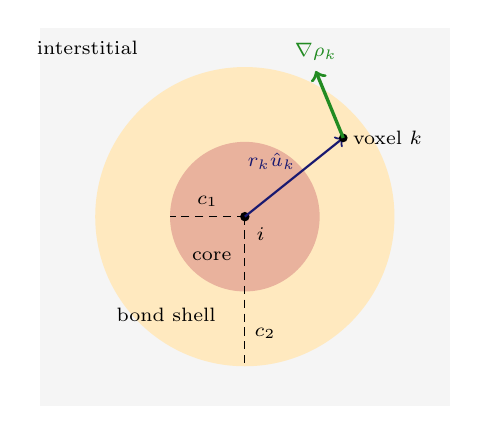
\begin{tikzpicture}[scale=1.0]
  \fill[gray!8] (-2.6,-2.4) rectangle (2.6,2.4);
  \fill[Orange!25] (0,0) circle (1.9);
  \fill[BrickRed!28] (0,0) circle (0.95);
  \fill[black] (0,0) circle (0.06);
  \node at (0.2,-0.22) {\scriptsize $i$};
  \node at (-2.0,2.15) {\scriptsize interstitial};
  \node at (-0.42,-0.5) {\scriptsize core};
  \node at (-1.0,-1.25) {\scriptsize bond shell};
  \draw[densely dashed] (0,0) -- (-0.95,0) node[pos=0.5,above]{\scriptsize $c_1$};
  \draw[densely dashed] (0,0) -- (0,-1.9) node[pos=0.78,right]{\scriptsize $c_2$};
  \coordinate (k) at (1.25,1.0);
  \draw[thick,->,MidnightBlue] (0,0) -- (k) node[pos=0.55,above left,inner sep=1pt]{\scriptsize $r_k\hat u_k$};
  \fill (k) circle (0.055);
  \node[right] at (k) {\scriptsize voxel $k$};
  \draw[very thick,->,ForestGreen] (k) -- ++(-0.35,0.85) node[above]{\scriptsize $\nabla\rho_k$};
\end{tikzpicture}

{\small Each voxel $k$ is measured from its nearest nucleus.}
\end{minipage}

\textbf{Degenerate cases.} A descriptor that is undefined for a special input (e.g.\ a perfectly
uniform density, or an empty shell) returns a documented constant, and a flag is set in the
metadata; it never returns a bare NaN.

\textbf{Numerical stability.} Descriptors whose value changed by more than about 10\% on the
dataset when the derivatives were taken by finite differences instead of FFT, or when the grid
was coarsened to 80\%, were dropped (see the end).

%=====================================================================
\section{Bonding descriptors (19)}

\subsection{Where the charge sits: radial moments and shell fractions}
The simplest picture of a solid is a set of atoms. These descriptors ask how far, on average, the
charge lies from its nearest nucleus, and how it is shared between the core, the bond shell and the
space in between.
\begin{descs}
\entry{m1}{\AA}{$\displaystyle m_1=\frac{\sumk\rho_k r_k}{\sumk\rho_k}$}{Mean distance of the charge from its nearest nucleus. Small for compact, core-dominated atoms; large for diffuse valence charge.}
\entry{m2}{\AA$^2$}{$\displaystyle m_2=\frac{\sumk\rho_k r_k^2}{\sumk\rho_k}$}{Second radial moment; weights the outer charge more strongly.}
\entry{sigma_r2}{\AA$^2$}{$\sigma_r^2 = m_2 - m_1^2$}{Radial spread of the charge about its mean distance.}
\entry{f_core, f_bond, f_int}{}{$\displaystyle f_{\rm shell}=\frac{\sum_{k\in\text{shell}}\rho_k}{\sumk\rho_k}$,\quad $f_{\rm core}+f_{\rm bond}+f_{\rm int}=1$}{Fraction of the charge in the core, bond and interstitial shells. A large $f_{\rm int}$ points to delocalized (metallic) charge between the atoms.}
\end{descs}

\subsection{Is the charge spherical? Gradient anisotropy}
Around an isolated, spherical atom the density gradient points straight at the nucleus. Bonds, lone
pairs and other distortions tilt it sideways. $\zeta$ measures the share of the gradient that is
\emph{not} radial.
\begin{descs}
\entry{zeta}{range $[0,1]$}{$\displaystyle \zeta = 1-\frac{\sumk|\nabla\rho_k\cdot\hat u_k|}{\sumk|\nabla\rho_k|}$}{0 for spherical, non-overlapping atoms; grows as the charge is pulled off the radial direction (directional bonding).}
\end{descs}

\subsection{Where charge is concentrated: the Laplacian}
Where $\nabla^2\rho<0$ the density is locally concentrated (higher than its surroundings), as in
atomic shells, covalent bonds and lone pairs; where $\nabla^2\rho>0$ it is depleted.
\begin{descs}
\entry{lnf}{}{$\displaystyle \mathrm{lnf}=\frac{1}{N_v}\sumk \mathbf 1[\nabla^2\rho_k<0]$}{Volume fraction of the cell where charge is concentrated.}
\entry{lnf_charge_weighted}{}{$\displaystyle \frac{\sum_{\nabla^2\rho_k<0}\rho_k}{\sumk\rho_k}$}{Fraction of the \emph{charge} in concentration regions. Less sensitive to the grid than \dn{lnf}, because low-density voxels carry little weight.}
\entry{lap_concentration}{}{$\displaystyle \frac{\sum_{\nabla^2\rho_k<0}|\nabla^2\rho_k|}{\sumk|\nabla^2\rho_k|}$}{On a periodic grid $\int\nabla^2\rho\,dV=0$ exactly, so this is always $1/2$. It carries no information and is kept only for completeness.}
\entry{lap_concentration_valence}{}{same ratio, restricted to $r_k>c_1$}{The informative version: the balance of concentration and depletion in the valence region, outside the cores.}
\end{descs}

\subsection{Shape of the bonds: ellipticity}
At a bond, the two Hessian eigenvalues across the bond are negative. If they are equal the bond is
cylindrical (a $\sigma$ bond); if they differ the charge is flattened, as in $\pi$ character.
The usual ellipticity $\varepsilon = \lambda_1/\lambda_2 - 1$ diverges as $\lambda_2\to 0$, so
pydemi uses its bounded form. Let $B=\{k \in \text{bond shell}: \lambda_2<0\}$.
\begin{descs}
\entry{ellip_bond_bounded_avg}{range $[0,1)$}{mean over $B$ of $\displaystyle 1-\frac{\lambda_2}{\lambda_1} = \frac{\varepsilon}{1+\varepsilon}$}{0 for a cylindrical bond; approaches 1 for strongly flattened charge. Each voxel's value is at most 1, so a few voxels with $\lambda_2\approx 0$ cannot dominate the mean.}
\end{descs}

\subsection{Weak interactions (NCI)}
Non-covalent interactions show up where the density is low and nearly flat, which a small reduced
gradient $s$ picks out. The sign of $\lambda_2$ separates attractive ($\lambda_2<0$) from repulsive
contacts. The NCI region is $\{k: s_k<0.5,\ \rho_k<0.05$ a.u.$\}$, where
$s=|\nabla\rho|\,/\,\big(2(3\pi^2)^{1/3}\rho^{4/3}\big)$.
\begin{descs}
\entry{f_NCI}{}{volume fraction of the NCI region}{How much of the cell holds weak-interaction density.}
\entry{NCI_attractive}{}{fraction of NCI voxels with $\lambda_2<0$}{Share of the weak interactions that are attractive.}
\entry{sign_lambda2_rho_mean}{e/bohr$^3$}{mean over the NCI region of $\mathrm{sign}(\lambda_2)\,\rho$}{Signed strength of the weak interactions: negative means mostly attractive.}
\end{descs}

\subsection{Electrostatics (Hartree potential)}
The Hartree potential energy of an electron is obtained from $\rho$ by one FFT,
$V(\mathbf G) = 4\pi k_e\,\rho(\mathbf G)/|\mathbf G|^2$, with $k_e=14.40$\,eV\,\AA. The cell average
is set to zero.
\begin{descs}
\entry{V_spread}{eV}{$\mathrm{std}_i\, V(\mathbf R_i)$ over the atomic sites}{How different the electrostatic environments of the atoms are; a rough signature of charge transfer.}
\entry{V_int_min}{eV}{$\min_{k\in\text{int}} V_k$}{Lowest potential in the interstitial region.}
\end{descs}

\subsection{Density in the bonds}
Neighbours: $j$ is a first-shell neighbour of $i$ if $|\mathbf R_{ij}|\le 1.1\,d_i$, where $d_i$ is
the distance from $i$ to its nearest neighbour. $\rho$ at each bond midpoint is obtained by exact
Fourier interpolation.
\begin{descs}
\entry{rho_mid_mean}{e/\AA$^3$}{mean of $\rho$ at the nearest-neighbour bond midpoints}{How much charge sits in the bonds: high for covalent bonds, low for ionic contacts.}
\entry{rho_mid_std}{e/\AA$^3$}{standard deviation of the same values}{How uneven the bonds are.}
\end{descs}

%=====================================================================
\section{Structural descriptors (19)}

\subsection{Connectivity: percolation}
Lower a threshold $c$ from the density maximum. At first the region $\{\rho>c\}$ consists of
isolated islands around the atoms. At some level the islands join into a path that runs through the
whole crystal along a lattice direction $\mathbf a_\alpha$ (it winds around the periodic cell).
\begin{descs}
\entry{rho_perc_a, rho_perc_b, rho_perc_c}{e/\AA$^3$}{$\rho_{\mathrm{perc},\alpha}=\max\{c:\ \{\rho>c\}\ \text{spans along}\ \mathbf a_\alpha\}$}{Density at the bottleneck of the best connecting path. High in metals, close to zero in ionic and molecular solids.}
\entry{perc_anisotropy}{}{$(\max_\alpha-\min_\alpha)\,\rho_{\mathrm{perc},\alpha}\,/\,\mathrm{mean}_\alpha\,\rho_{\mathrm{perc},\alpha}$}{Whether the charge connects equally well in all three directions (0), or better along some (layered or chain-like structures).}
\end{descs}

\subsection{Peaks and valleys: the critical-point census}
Counts are divided by the cell volume, so they are per \AA$^3$.
\begin{descs}
\entry{n_max, n_min}{1/\AA$^3$}{voxels higher (lower) than all 26 neighbours, divided by $V$}{Local maxima (typically at or near the nuclei) and minima (centres of the voids).}
\entry{n_NNM}{1/\AA$^3$}{maxima farther than $0.8$\,\AA\ from every nucleus, divided by $V$}{Non-nuclear maxima: charge pooled away from the atoms, e.g.\ in electrides or some metals.}
\entry{Q_NNM}{}{(charge in the steepest-ascent basins of those maxima)$/Q_{\rm tot}$}{How much charge the non-nuclear maxima hold.}
\end{descs}

\subsection{The density floor}
\begin{descs}
\entry{rho_min}{e/\AA$^3$}{$\min_k\rho_k$}{Lowest density in the cell. In a CHGCAR (a PAW pseudo-density) this is often slightly negative and near a nucleus, not in the voids.}
\entry{rho_min_ratio}{}{$\rho_{\min}/\langle\rho\rangle$}{The same, relative to the mean density.}
\entry{rho_int_mean}{e/\AA$^3$}{mean of $\rho$ over the interstitial shell}{How much charge fills the space between the atoms.}
\end{descs}

\subsection{Directionality: the charge-anisotropy tensor}
Averaging the gradient's directions over the whole cell gives a $3\times3$ tensor with trace 1:
\[
T_{ab}=\frac{\sumk \partial_a\rho_k\,\partial_b\rho_k}{\sumk |\nabla\rho_k|^2},\qquad
\text{eigenvalues } t_1\le t_2\le t_3,\quad t_1+t_2+t_3=1 .
\]
\begin{descs}
\entry{T_eigenvalues_t1, _t2, _t3}{}{the sorted eigenvalues of $T$}{All $1/3$ when the gradients point equally in all directions (e.g.\ any cubic crystal). Unequal values show that the density varies more along some directions, as in layered or chain structures.}
\entry{charge_FA}{range $[0,1]$}{$\displaystyle \mathrm{FA}=\sqrt{\tfrac32}\,\frac{\lVert T-\tfrac13 I\rVert_F}{\lVert T\rVert_F}$}{Fractional anisotropy: one number for how far $T$ is from isotropic. 0 when isotropic; 1 when every gradient is parallel.}
\end{descs}

\subsection{Information content}
These treat the normalized density $\rhot = \rho/N_e$ (with $N_e=\int\rho\,dV$) as a probability
distribution over the cell. Each is normalized by the cell volume, which makes it intensive.
\begin{descs}
\entry{shannon_entropy}{range $\le 0$}{$\displaystyle S=-\!\int\rhot\ln\rhot\,dV-\ln V$}{How spread out the charge is: 0 for a uniform density, more negative as the charge concentrates on the atoms.}
\entry{disequilibrium}{range $\ge 1$}{$\displaystyle D = V\!\int\rhot^{\,2}\,dV$}{How far the charge is from uniform: 1 for a uniform density, larger when it is concentrated.}
\entry{LMC_complexity}{}{$C = D\,e^{S}$}{L\'opez-Ruiz--Mancini--Calbet complexity. It balances order against disorder and equals 1 for a uniform density.}
\entry{fisher_information}{1/bohr$^2$}{$\displaystyle I=\int\frac{|\nabla\rhot|^2}{\rhot}\,dV$}{Sharpness of the density: large when it changes steeply (compact cores, strong localization).}
\end{descs}

%=====================================================================
\section{Heterogeneity descriptors (18)}
The descriptors above describe the whole cell. These ask \emph{how different the atoms are}. Each
voxel is assigned to an atom (default: its nearest nucleus, i.e.\ Voronoi cells; smooth partitions give fractional weights). Then three per-atom
quantities are computed, each the per-atom version of a bonding descriptor ($w_i(k)=1$ if voxel $k$
belongs to atom $i$):
\[
m_1^{(i)}=\frac{\sum_k w_i(k)\rho_k r_{ik}}{\sum_k w_i(k)\rho_k},\qquad
f_{\rm bond}^{(i)}=\frac{\sum_{c_1<r_{ik}\le c_2} w_i(k)\rho_k}{\sum_k w_i(k)\rho_k},\qquad
\zeta^{(i)}=1-\frac{\sum_k w_i(k)|\nabla\rho_k\cdot\hat u_{ik}|}{\sum_k w_i(k)|\nabla\rho_k|}.
\]
For each $X\in\{m_1, f_{\rm bond}, \zeta\}$, six statistics over the atoms are reported (18 in
total). Let $x_e$ be the fraction of sites of element $e$, $\bar X_e$ the mean over the sites of
element $e$, and $\bar X$ the mean over all sites.

\begin{center}
\renewcommand{\arraystretch}{1.25}
\begin{tabularx}{\linewidth}{@{}l l X@{}}
\toprule
descriptor & definition & meaning\\
\midrule
\dn{X_site_std} & $\mathrm{std}_i X^{(i)}$ & overall spread between atoms\\
\dn{X_site_range} & $\max_i X^{(i)}-\min_i X^{(i)}$ & the most extreme difference\\
\dn{X_site_max}, \dn{X_site_min} & $\max_i X^{(i)}$, $\min_i X^{(i)}$ & the extreme atoms\\
\dn{X_within_element_var} & $\sum_e x_e\,\mathrm{Var}_{i\in e}X^{(i)}$ & atoms of the \emph{same} element in different environments\\
\dn{X_between_element_var} & $\sum_e x_e\,(\bar X_e-\bar X)^2$ & differences \emph{between} elements\\
\bottomrule
\end{tabularx}
\end{center}
The last two split the variance exactly, $\mathrm{Var}_i X = \text{within} + \text{between}$ (as in
one-way ANOVA). The within-element variance is undefined (NaN, flagged) when no element has two or
more sites. The between-element variance is 0 (flagged) for a single-element crystal. Units are
those of $X$ (\AA\ for $m_1$, squared for the variances; $f_{\rm bond}$ and $\zeta$ are
dimensionless).

%=====================================================================
\section*{Summary}
\begin{center}
\renewcommand{\arraystretch}{1.05}
\small
\begin{tabularx}{\linewidth}{@{}l c X@{}}
\toprule
group & $n$ & what it captures\\
\midrule
moments and shells & 6 & where the charge sits relative to the nuclei\\
gradient anisotropy & 1 & how non-spherical the atoms are\\
Laplacian & 4 & where charge is concentrated or depleted\\
ellipticity & 1 & cylindrical vs.\ flattened bonds\\
NCI & 3 & weak, non-covalent interactions\\
Hartree potential & 2 & electrostatic environment of the atoms\\
bond midpoints & 2 & charge in the bonds\\
\midrule
percolation & 4 & how well the charge connects through the crystal\\
critical points & 4 & peaks, valleys and non-nuclear maxima\\
density floor & 3 & charge in the voids\\
anisotropy tensor & 4 & directionality of the whole density\\
information measures & 4 & spread, concentration and sharpness\\
\midrule
heterogeneity & 18 & differences between atoms, within and between elements\\
\midrule
\textbf{total} & \textbf{56} & \\
\bottomrule
\end{tabularx}
\end{center}
\textbf{Defaults:} $c_1=0.8$\,\AA, $c_2=1.5$\,\AA; FFT derivatives; nearest-atom partition; \texttt{featurize} returns all 56.

\textbf{Not included, and why.}
\begin{itemize}[leftmargin=1.4em,itemsep=0.3ex,topsep=0.3ex]
\item \emph{ELF and local energy densities} ($g$, $v$, $H$): a CHGCAR has no orbitals, so both
  would have to be estimated from the PAW pseudo-density with a density-only approximation of the
  kinetic energy. The results are not the true quantities.
\item \emph{Mean and spread of the unbounded ellipticity $\varepsilon$}: they diverge as
  $\lambda_2\to0$. On the dataset the mean changed by a median 22\% (FD4 vs.\ FFT derivatives)
  and the spread by 67\%; the bounded form above changed by 0.2\%.
\item \emph{Saddle-point counts}: they changed by a median 17--20\% when the grid was coarsened
  to 80\%.
\end{itemize}

\end{document}
